\documentclass[14pt,a4paper]{extarticle}
\usepackage{../templates/preamble}

\newcommand{\reportof}{практической работе №4}
\newcommand{\theme}{Методы нахождения производной.}

\begin{document}
\begin{titlepage}
    \begin{center}
        {\bfseries
        МИНОБРНАУКИ РОССИИ\par
        САНКТ-ПЕТЕРБУРГСКИЙ ГОСУДАРСТВЕННЫЙ\par
        ЭЛЕКТРОТЕХНИЧЕСКИЙ УНИВЕРСИТЕТ\par
        <<ЛЭТИ>> ИМ. В.И. УЛЬЯНОВА (ЛЕНИНА)\par
        Кафедра \department

        \vspace{0.23\textheight}
        ОТЧЁТ\par
        по \reportof\par
        по дисциплине <<\discipline>>\par
        Тема: \theme
        \vspace{0.28\textheight}
        }
        \begin{table}[!ht]
            \begin{tabularx}{\textwidth}{p{60mm}X>{\centering\arraybackslash}p{45mm}}
                Студент гр. 4352 & \_\_\_\_\_\_\_\_\_\_\_\_\_\_\_\_\_\_\_\_ & {Даричев Е. М.} \\ [5.4mm]  % Line height
                Преподаватель    & \_\_\_\_\_\_\_\_\_\_\_\_\_\_\_\_\_\_\_\_ & {\teacher} \\ [5.4mm]
            \end{tabularx}
        \end{table}

        Санкт-Петербург\par
        \yyear
    \end{center}
\end{titlepage}
\setcounter{page}{2}

\section*{Цель работы}
        Изучить основные методы нахождения производных.


\section*{Отчёт о проделанной работе}
        В первом задании необходимо найти промежутки возрастания и
убывания нескольких функций с помощью их производных. Для этого воспользуемся
правилами нахождения производных. Воспользовавшись кодом из предыдущего
практического задания, узнаем промежутки знакопостоянства и нули
производной и построим графики функций. Код приведён на рисунке \ref{fig:4.1-code}, результаты
--- на рисунке \ref{fig:4.1-result}.

\begin{figure}[h!]
    \centering
    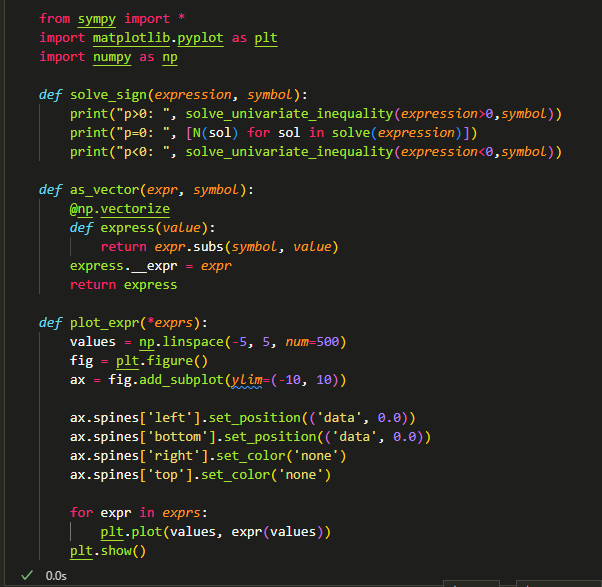
\includegraphics[width=0.7\linewidth]{figures/1-code.png}
    \caption{Расчёт промежутков знакопостоянства и отображение функций}
    \label{fig:4.1-code}
\end{figure}

\newpage

\begin{figure}[ht!]
    \centering
    \begin{subfigure}{.333\textwidth}
        \centering
        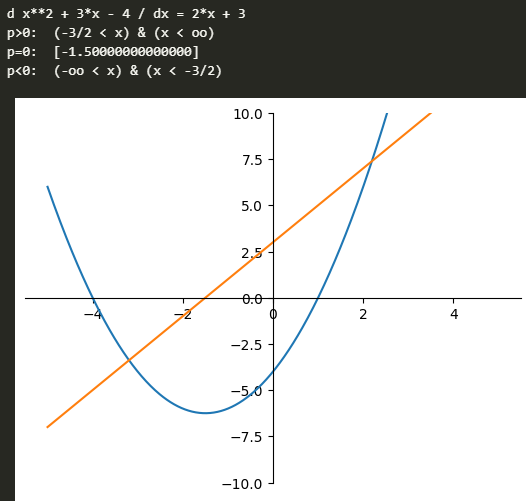
\includegraphics[width=\linewidth]{figures/1-1.png}
    \end{subfigure}%
    \begin{subfigure}{.333\textwidth}
        \centering
        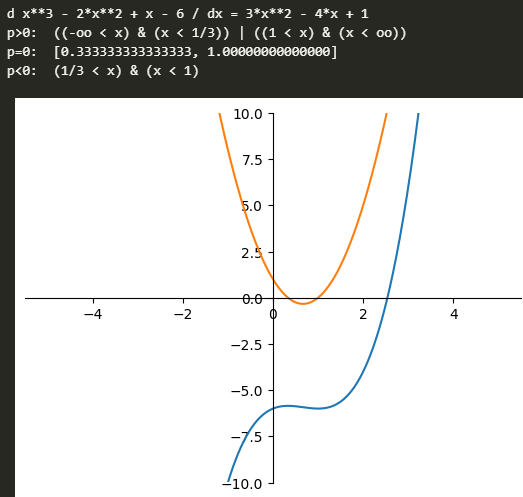
\includegraphics[width=\linewidth]{figures/1-2.png}
    \end{subfigure}%
    \begin{subfigure}{.333\textwidth}
        \centering
        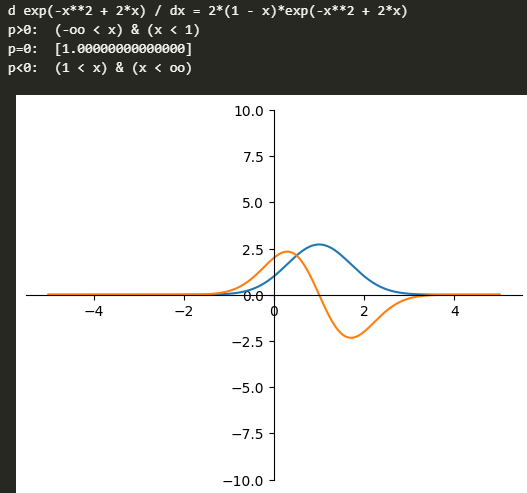
\includegraphics[width=\linewidth]{figures/1-3.png}
    \end{subfigure}%
    \caption{Результаты задания 4.1}
    \label{fig:4.1-result}
\end{figure}


Во второй части необходимо найти производные функций. Воспользуемся для этого
функционалом $sympy$, а именно --- функцией \textit{diff}, которая позволяет найти
производную выражения относительно переменной. Результаты задания 4.2 см.рис. \ref{fig:4.2},
результаты задания 4.3 --- рис. \ref{fig:4.3}.


\begin{figure}[ht!]
    \centering
    \begin{subfigure}{.5\textwidth}
        \centering
        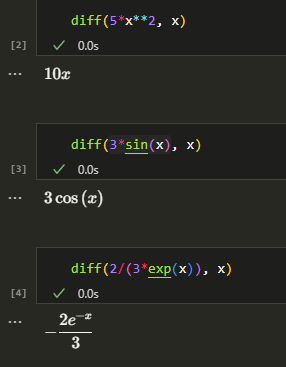
\includegraphics[width=0.7\linewidth]{figures/2-1.png}
    \end{subfigure}%
    \begin{subfigure}{.5\textwidth}
        \centering
        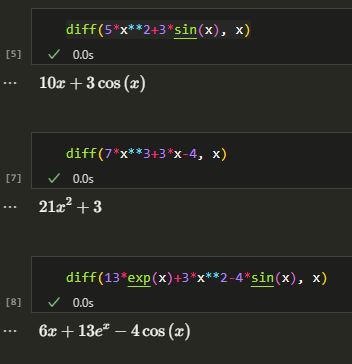
\includegraphics[width=0.7\linewidth]{figures/2-2.png}
    \end{subfigure}%
    \caption{Результаты задания 4.2}
    \label{fig:4.2}
\end{figure}
\newpage
\begin{figure}[ht!]
    \centering
    \begin{subfigure}{.5\textwidth}
        \centering
        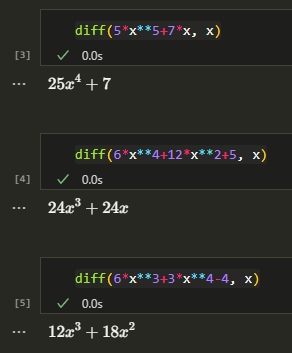
\includegraphics[width=0.7\linewidth]{figures/3-1.png}
    \end{subfigure}%
    \begin{subfigure}{.5\textwidth}
        \centering
        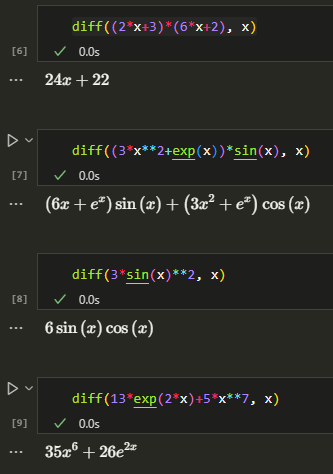
\includegraphics[width=0.7\linewidth]{figures/3-2.png}
    \end{subfigure}%
    \caption{Результаты задания 4.3}
    \label{fig:4.3}
\end{figure}


\section*{Вывод}

        В ходе выполнения работы я вспомнил правила нахождения производных,
познакомился с символическим поиском производной с помощью \textit{sympy}.

\end{document}